\documentclass{beamer}
\usepackage{tcolorbox}
\usepackage{hyperref}
\usepackage{../notation}

%\beamerdefaultoverlayspecification{<+->}
% \newcommand{\data}{\mathcal{D}}
% \newcommand\Item[1][]{%
% 	\ifx\relax#1\relax  \item \else \item[#1] \fi
% 	\abovedisplayskip=0pt\abovedisplayshortskip=0pt~\vspace*{-\baselineskip}}

\graphicspath{ {imgs/} }

\usetheme{metropolis}           % Use metropolis theme


\title{Convex Functions}
\date{\today}
\author{Nipun Batra}
\institute{IIT Gandhinagar}
\begin{document}
	\maketitle

	\begin{frame}{Definition}
	\begin{itemize}
	\item Convexity is defined on an interval [$\alpha,\beta$]
	\item The line segment joining $(a,f(a)) and (b, f(b))$ should be \textit{above or on} the function $f$ for all points in interval  [$\alpha,\beta$].
	\end{itemize}
	\begin{center}
	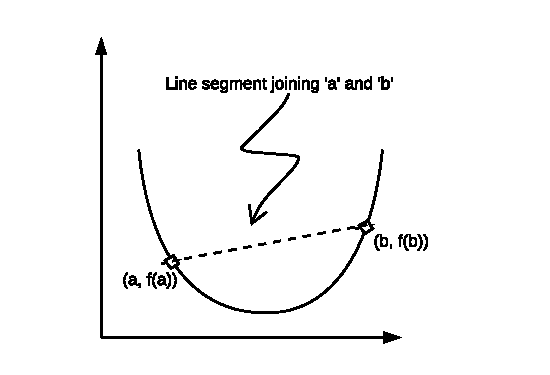
\includegraphics[scale=0.8]{fig1}
	\end{center}
	\end{frame}
	
	\begin{frame}{Example: $y = x^2$}
	Convex on the entire real line i.e. $(-\infty, \infty)$
	\begin{center}
	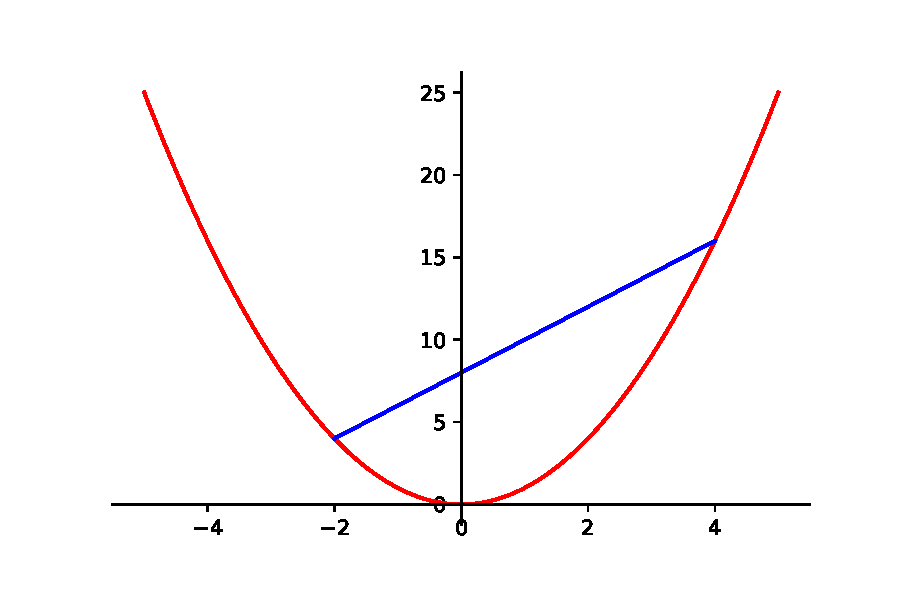
\includegraphics[scale=0.5]{y-x2}
	\end{center}
	\end{frame}

	\begin{frame}{Example: $y = |x|$}
	Convex on the entire real line i.e. $(-\infty, \infty)$
	\begin{center}
	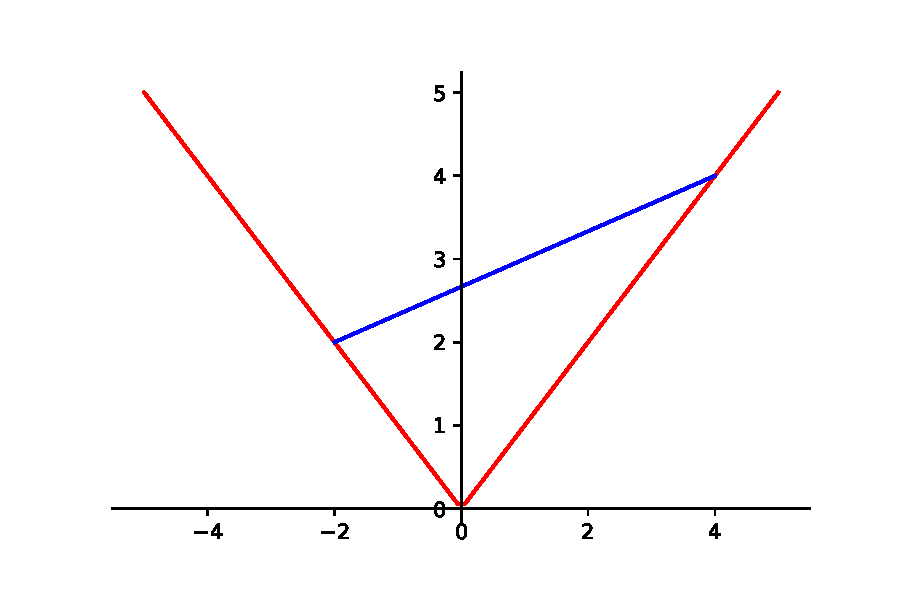
\includegraphics[scale=0.5]{y-absx}
	\end{center}
	\end{frame}

	\begin{frame}{Example: $y = e^x$}
	Convex on the entire real line i.e. $(-\infty, \infty)$
	\begin{center}
	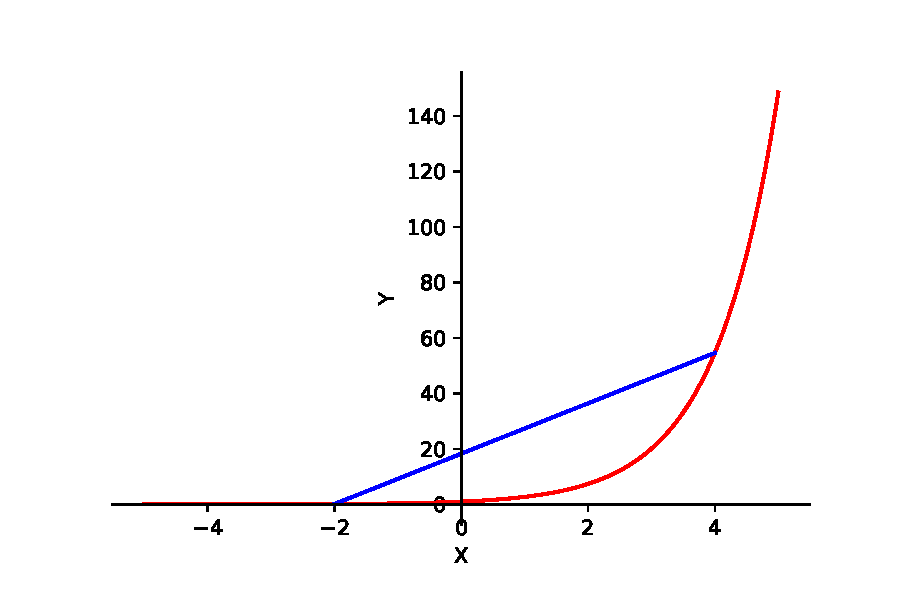
\includegraphics[scale=0.5]{y-ex}
	\end{center}
	\end{frame}

	\begin{frame}{Example: $y = log_ex$}
	Not convex on the entire real line i.e. $(-\infty, \infty)$
	\begin{center}
	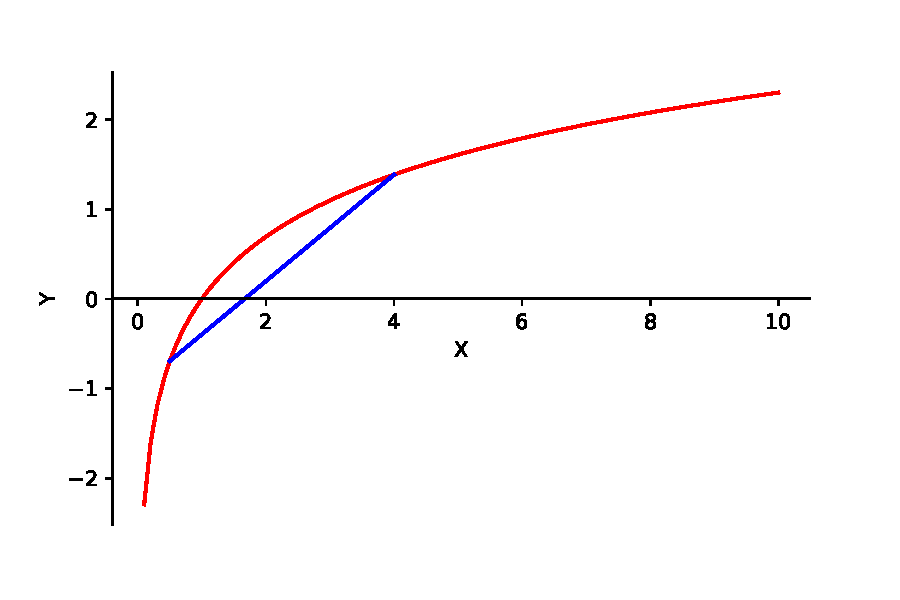
\includegraphics[scale=0.5]{y-logx}
	\end{center}
	\end{frame}

	\begin{frame}{Example: $y = x^3$}
	It is convex for the interval $[0,\infty)$
	\begin{center}
	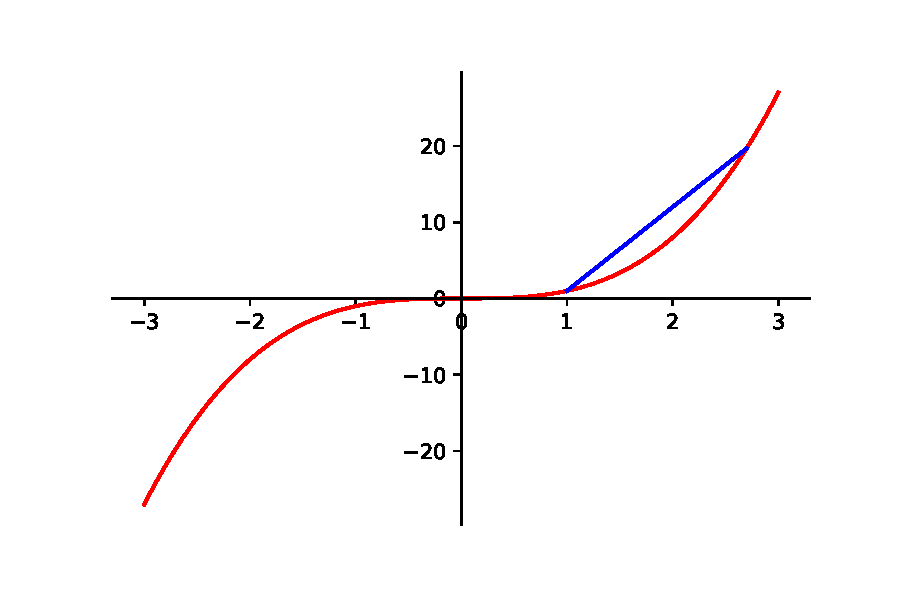
\includegraphics[scale=0.5]{y-x3_pos}
	\end{center}
	\end{frame}

	\begin{frame}{Example: $y = x^3$}
	It is concave for the interval $(-\infty, 0]$
	\begin{center}
	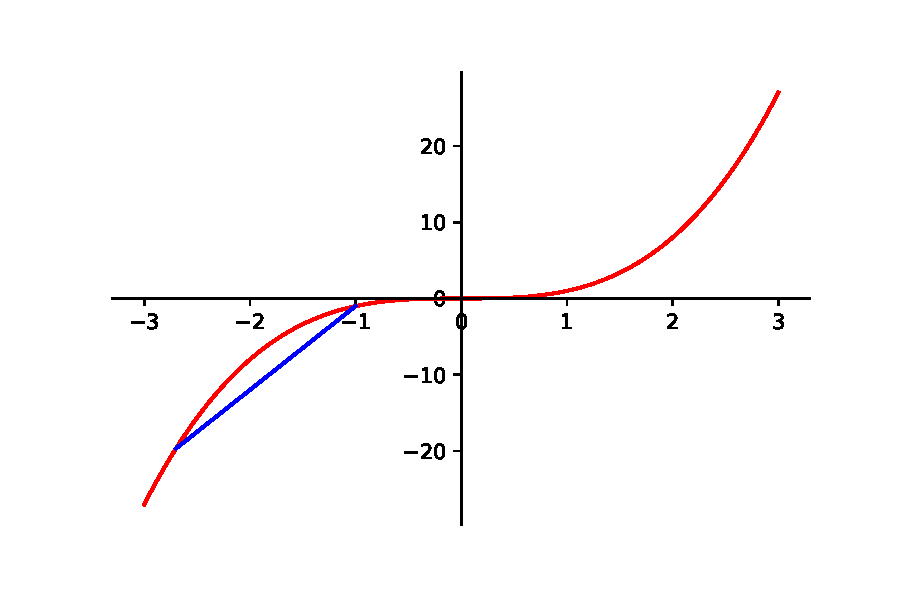
\includegraphics[scale=0.5]{y-x3_neg}
	\end{center}
	\end{frame}

	\begin{frame}{Example: $y = x^3$}
	But, it is not convex for the interval $(-\infty, \infty)$
	\begin{center}
	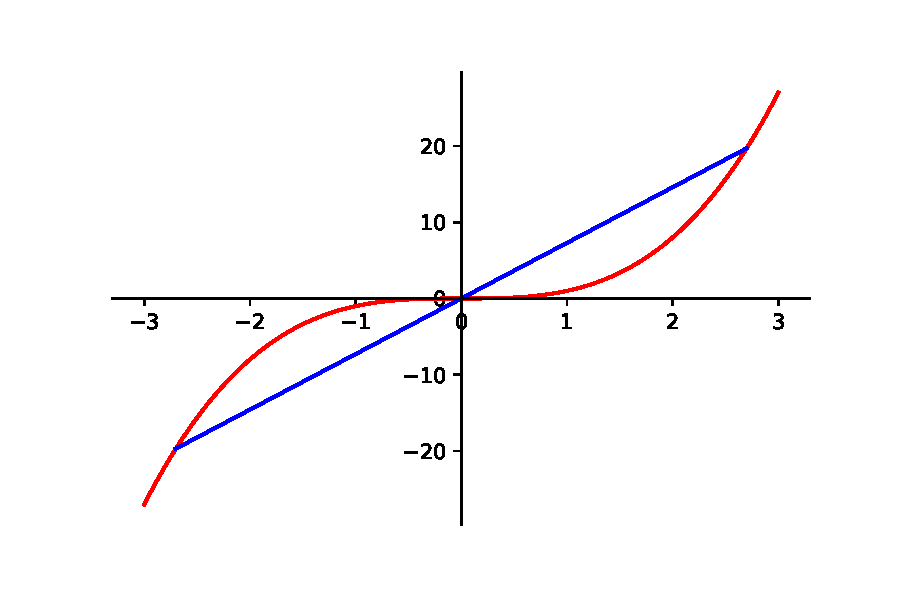
\includegraphics[scale=0.5]{y-x3}
	\end{center}
	\end{frame}

	\begin{frame}{Mathematical Formulation}
	Function $f$ is convex on set $X$, if $\forall x_1,x_2 \in X$ and $\forall t \in [0,1]$
	\begin{center}
	$f(tx_1 + (1-t)x_2) \leq tf(x_1) + (1-t)f(x_2)$\\
	\vspace{0.4cm}
	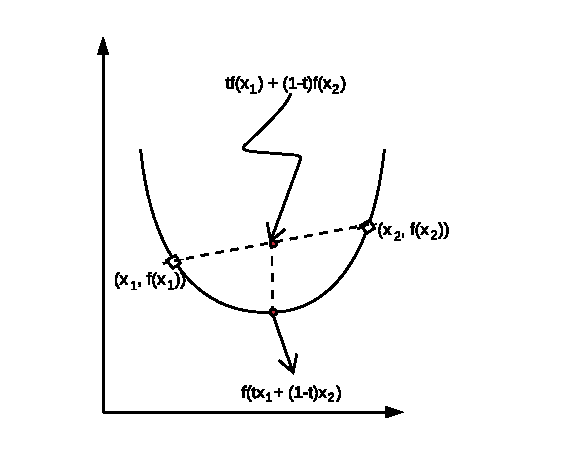
\includegraphics[scale=0.75]{proof_notation_fig}
	\end{center}
	\end{frame}


	\begin{frame}{Question: Prove that $f(x) = x^2$ is convex}
	\end{frame}

	\begin{frame}{Question: Prove that $f(x) = x^2$ is convex}
	\only<1-4>{To prove:
	\begin{center}
	$f(tx_1 + (1-t)x_2) \leq tf(x_1) + (1-t)f(x_2)$
	\end{center}
	}
	\only<2-4>{LHS = $f(tx_1 + (1-t)x_2)$ \hspace{0.5cm}=  $t^2x_1^2 + (1-t)^2x_2^2 + 2t(1-t)x_1x_2$\\
	RHS = $ tf(x_1) + (1-t)f(x_2)$ =  $tx_1^2 + (1-t)x_2^2$\\}
	\vspace{0.3cm}
	\only<3-4>{Here,\\
	LHS - RHS = $(t^2 -t)x_1^2 + [(1-t)^2 - (1-t)]x_2^2 + 2t(1-t)x_1x_2$ \\
	\hspace{1.8cm}               = $(t^2 - t)x_1^2 + (t^2 - t)x_2^2 - 2(t^2 - t)x_1x_2$\\
	\hspace{1.8cm}		      = $(t^2 - t)(x_1 - x_2)^2$ \\
	\vspace{0.3cm}
	}
	\only<4>{Here, $(t^2 - t) \leq 0$ since $t \in [0,1]$ and $(x_1 - x_2)^2 \geq 0$\\
	Hence, LHS -RHS $\leq$ 0\\
	Hence LHS $\leq$ RHS\\
	Hence proved.
	}
	\end{frame}


	\begin{frame}{Alternative ways to prove convexity}
	The Double-Derivative Test\\
	\vspace{1cm}
	If f''(x) $>$ 0, the function is  convex.\\
	\vspace{1cm}
	For example,\\
	\vspace{1cm}
	$\dfrac{\partial ^2( x^2)}{\partial x^2} = 2 > 0 \Rightarrow x^2$ is a Convex function.\\  
	\end{frame}

	\begin{frame}{Alternative ways to prove convexity}
	The double derivate test for multi-parameter function is equal to using the Hessian Matrix\\
	\vspace{1cm}
	A function $f(x_1,x_2,\dots,x_n)$ is convex iff its $n \times n$ Hessian Matrix is positive semidefinite for all posible values of $(x_1,x_2,\dots, x_n)$\\
	\begin{equation*}
\mathbf{H}=\left[\begin{array}{cccc}
{\frac{\partial^{2} f}{\partial x_{1}^{2}}} & {\frac{\partial^{2} f}{\partial x_{1} \partial x_{2}}} & {\cdots} & {\frac{\partial^{2} f}{\partial x_{1} \partial x_{n}}} \\
{\frac{\partial^{2} f}{\partial x_{2} \partial x_{1}}} & {\frac{\partial^{2} f}{\partial x_{2}^{2}}} & {\cdots} & {\frac{\partial^{2} f}{\partial x_{2} \partial x_{n}}} \\
{\vdots} & {\vdots} & {\ddots} & {\vdots} \\
{\frac{\partial^{2} f}{\partial x_{n} \partial x_{1}}} & {\frac{\partial^{2} f}{\partial x_{n} \partial x_{2}}} & {\cdots} & {\frac{\partial^{2} f}{\partial x_{n}^{2}}}
\end{array}\right]
\end{equation*}
	\end{frame}


	\begin{frame}{Alternative ways to prove convexity}
	Show that $f(x_1,x_2) = x_1^2 + x_2^2$ is convex.\\
	\vspace{1cm} 
	\only<2->{
	\begin{equation*}
	H = 
	\begin{bmatrix}
		\dfrac{\partial ^2( x_1^2 + x_2^2)}{\partial x_1^2} & \dfrac{\partial ^2( x_1^2 + x_2^2)}{\partial x_1\partial x_2} \\
		 \dfrac{\partial ^2( x_1^2 + x_2^2)}{\partial x_2\partial x_1} & \dfrac{\partial ^2( x_1^2 + x_2^2)}{\partial x_2^2} \\
	\end{bmatrix}
	= 
	\begin{bmatrix}
		2 & 0 \\
		0 & 2\\
	\end{bmatrix}
	\end{equation*}\\
	}
	\only<3->{
	\vspace{1cm}
	Eigen Values of H are 2 and 2 $> 0 \Rightarrow$ H is positive semi-definite.\\
	Hence, $f(x_1,x_2) = x_1^2 + x_2^2$ is convex. 
	}
	\end{frame}

	\begin{frame}{Convexity of linear least squares}
	Prove the convexity of linear least squares i.e. $f(\theta) = ||y - X\theta||^2$\\
	\vspace{0.5cm}
	\only<2->{
	We will use the double derivate (Hessian)\\
	\vspace{0.5cm}
	}
	\only<3->{
	$\dfrac{df}{d\theta} = \dfrac{d(||y^2||  - 2y^TX\theta + ||X\theta||^2)}{d\theta} = -2y^TX + 2(X\theta)^TX$\\
	\vspace{0.5cm}
	}
	\only<4->{
	$\dfrac{d^2f}{d\theta^2} = H = 2X^TX$\\
	\vspace{1cm}
	}
	\only<5->{
	$X^TX$ is positive semi-definite for any $X \in \mathbb{R}^{m\times n}$.\\
	Hence, linear least squares function is convex.
	}
	\end{frame}


	\begin{frame}{Properties of Convex Functions}
	\begin{itemize}
	\only<1-3>{\item If $f(x)$ is convex, then $kf(x)$ is also convex, for some constant $k$}
	\only<2-3>{\item If $f(x)$ and $g(x)$ are convex, then $f(x) + g(x)$ is also convex.}
	\end{itemize}
	
	
	\only<3>{Using this we can say that,
	\begin{itemize}
	\item $(y-x\theta)^T(y-x\theta) + \theta^T\theta$ is convex 
	\item $(y-x\theta)^T(y-x\theta) + |\theta|$ is convex 
	\end{itemize}
	}
	\end{frame}

\end{document}